\documentclass[a4paper,french]{report}
\usepackage[utf8]{inputenc}
\usepackage{graphicx}
\usepackage{algorithm}
\usepackage{algorithmic}
\usepackage[left=2cm,right=2cm,top=2cm,bottom=2cm]{geometry}
\usepackage{titlesec}
\titleformat{\chapter}[hang]{\Huge\bfseries}{\thechapter{ - }}{0pt}{\Huge\bfseries}
\usepackage{babel}
\setlength{\parindent}{20pt}

\begin{document}
	\Large
	PRIN Guillaume \hfill Année 2015-2016\newline
	\begin{center}
		\Huge
		Projet : Génération de dégradations physiques sur les modèles 3D
	\end{center}
	\vspace*{2cm}
	\begin{center}
		\Huge
		\underline{Rapport de projet}
	\end{center}
	\begin{center}
	
\includegraphics
	{ulco.png}
	\end{center}
	\vfill
	Tuteurs de projet : 
	\begin{itemize}
		\item Christophe Renaud
		\item François Rousselle
	\end{itemize}
	\newpage
	\chapter*{Remerciements}
			Je souhaite avant tout remercier M. Rousselle et M. Renaud, qui ont accepté que je travaille avec eux sur ce projet, et qui m'ont beaucoup aidé à sa réalisation. Je remercie aussi M. Verel qui, avec mes collègues, nous a donné de nombreux conseils quant à la réalisation de ce rapport, autant sur le fond que sur la forme.
	\tableofcontents
	\newpage
	\chapter{Positionnement du projet}
		\section{Rappel : Contexte et définition du problème}
			Dans le cadre de reconstitutions virtuelles historiques,  le challenge de l'équipe pluridisciplinaire réunie (informaticiens et historiens) consiste à s'approcher au plus près de la réalité historique de l'environnement reconstruit. Au travers de recherches approfondies dans divers fonds d'archives, les historiens apportent ainsi des connaissances fondamentales à la reconstruction 3D des environnements ciblés, permettant ensuite une visualisation plus ou moins réaliste et/ou plus ou moins interactive de ces environnements, pour des applications diverses à destination des chercheurs ou du grand public.. \par
			Un défaut fréquent de ces reconstitutions réside dans le fait qu'ils apparaissent comme neufs, ce qui est clairement préjudiciable à leur interprétation dans leur contexte historique. Un travail complémentaire, effectué par des infographistes, consiste alors à introduire des dégradations dans ces environnements, provenant tant de causes naturelles (vent, pluie, etc.) que humaines (usures dues aux passages répétés, chocs, déprédations volontaires, etc.). \par
			L'objectif est de se focaliser sur un type particulier de dégradation, lié à l'usure et aux chocs reçus par les pierres qui apparaissent dans le bâti reconstruit, qu'il s'agisse de marches d'escalier ou des pierres des murs. Le travail à réaliser consistera à développer le code d'une méthode existante et à tester son utilisation dans le cadre d'une reconstitution du Pont Notre Dame en 1720.
		\section{Encadrants}
			Je suis encadré pendant ce projet par M. Christophe Renaud, directeur du LISIC et responsable de l'équipe IMAP (Images et Apprentissage) du laboratoire de recherche, et par M. Rousselle, maître de conférences, enseignant-chercheur à l'IUT de Calais-Boulogne, et membre de l'équipe IMAP du laboratoire de recherche.
		\section{L'état initial}
			Le pont Notre Dame a déjà été intégralement modélisé sous 3DsMax par M. Rousselle, et m'a été fourni au format Wavefront obj à des fins de tests. 
		\section{Durée du projet}
			La période libre de projet s'étale du 18 avril au 05 juin 2016. Toutefois, comme mentionné par M. Fabien Teytaud, responsable du Master 1 Informatique ISIDIS, il est fort recommandé de commencer le projet dès le mois de janvier.
		\section{Les outils mis en place}
			Une boite de dépôt github a été créée pour l'occasion, à l'adresse suivante :  https://github.com/guil-prin/notreDame . Régulièrement mise à jour, vous pouvez y trouver l'évolution du développement (dossier "dev"), les documents produits pour le projet (dont ce rapport, dans le dossier "documentation"), et les sources finales (dossier "sources"). Les descriptions fonctionnelles du projet sont d'ailleurs dans le cahier des charges fourni le 25 avril. \par
			Un disque dur avec un système d'exploitation Debian vierge installé m'a été gracieusement prêté par Nathalie Ramat, responsable du parc informatique de l'ULCO, afin que je puisse bénéficier du statut d'administrateur sur mon pc, et que je puisse donc installer les outils nécessaires au développement du projet. \par
			Une bibliothèque c++ a aussi été mise en place : CGAL. Disponible sur le site http://www.cgal.org/, elle permet de travailler sur une structure 3D avec des outils fournis pour définir un objet 3D et ses composants (arêtes, sommets, faces). La recherche de cette bibliothèque a été une partie du travail préliminaire au projet.
			
	\chapter{Travaux préliminaires}
		\section{Étude documentaire}
			Deux notes de recherche m'ont été confiés par M. Renaud lors de notre premier entretien : 
				\begin{itemize}
					\item Surface Aging by Impacts \cite{PPD01}
					\item Modeling cracks and fractures \cite{Liris-6004}
				\end{itemize}\par
			Il m'a aussi expliqué le but du projet : le modèle 3D déjà créé est terminé, mais il s'avère être "trop beau" par rapport à la réalité. En effet, les bâtiments modélisés s'avèrent en réalité avoir environ une centaine d'années d'après les historiens avec qui ils travaillent. Le but est donc de vieillir le modèle 3D afin de le prendre plus proche de la réalité. \par
			Il m'a donc été demandé à ce moment de consulter ces papiers de recherche, et plus particulièrement Surface Aging by Impacts \cite{PPD01}. J'ai eu plusieurs réunions avec M. Rousselle pour discuter de ce papier en détail. J'ai eu, à la demande de ce dernier, à réaliser une synthèse personnelle de ce papier afin de me faire comprendre la démarche d'un document scientifique (un cours d'initiation à la recherche a été enseigné par M. Verel à ce propos, mais n'a eu lieu que après cette réunion). Cette synthèse est disponible dans le dossier documentation du projet. \par
			Une troisième note de recherche me sera fournie au début de la période de projet, Real-Time Relief Mapping on Arbitrary Polygonal Surfaces \cite{Policarpo:2005:RRM:1053427.1053453}. Bien que consultée, elle ne sera pas intéressante pour cette période de projet.
			
		\section{Recherche de bibliothèques}
			Au cours de ces entretiens, il m'a aussi été demandé de rechercher des bibliothèques c++ afin d'éviter à devoir tout coder. En effet, la modélisation 3D est un domaine extrêmement en vogue à l'heure actuelle (que ce soit pour des simulations historiques, des modélisations de prototypes, des créations de jeux vidéos, ...), et de nombreuses personnes ont déjà travaillé dans ce domaine. Deux bibliothèques ont ainsi été trouvées par mes soins : les bibliothèques Assimp (http://www.assimp.org/) et Magnum (http://mosra.cz/blog/magnum.php), don la dernière n'a pas retenu notre attention. par la suite, M. Rousselle s'est rappelé d'un projet graphique réalisé quelques années auparavant par deux anciens étudiants, et ils avaient utilisé la bibliothèque CGAL. Cette dernière répondant à nos besoins, elle a été gardée pour le développement, tout en mettant de côté Assimp s'il s'avère que CGAL montre des limites. 
		
	\chapter{Recherche et Développement}
		\section{Comment vieillir des pierres ?}
			L'idée générale du vieillissement est de réaliser de nombreux petits impacts sur la surface à vieillir, afin que le cumul de ces impacts donne une sensation d'usure sur l'objet 3D. Surface Aging by Impacts \cite{PPD01} explique en détail une théorie de l'idée. Dans le cadre de ce projet, les étapes de la réalisation d'un impact sont les suivantes : 
			\begin{algorithm}[H]
				\caption{Réaliser un impact}
				\begin{algorithmic}[1]
					\STATE Charger l'objet 3D sur lequel travailler
					\REPEAT
						\REPEAT
							\STATE Chercher la/les face(s) sur laquelle/lesquelles le point d'impact aura lieu
							\IF{le point est sur une face}
								\STATE Affiner le maillage de la face qui sera impactée
							\ELSIF{le point est sur une arête}
								\STATE Affiner le maillage de l'arête et des faces adjacentes qui seront impactées
							\ELSIF{le point est sur un sommet}
								\STATE Affiner le maillage des arêtes et des faces adjacentes qui seront impactées
							\ELSE
								\STATE Arrêter le processus
							\ENDIF
						\UNTIL{surface de la face à impacter en dessous d'un certain seuil}
						\STATE Réaliser l'impact
					\UNTIL{impact souhaité obtenu}
					\STATE Enregistrer l'objet 3D réalisé
				\end{algorithmic}
			\end{algorithm}
			
			
		\section{Lire et écrire un objet 3D}
			\subsection{Structure d'un objet 3D au format OBJ}
				\subsubsection{Définition (Wikipédia)}
				OBJ est un format de fichier contenant la description d'une géométrie 3D. Il a été défini par la société Wavefront Technologies dans le cadre du développement de son logiciel d'animation Advanced Visualizer. Ce format de fichier est ouvert et a été adopté par d'autres logiciels 3D pour des traitements d'import / export de données.
				\subsubsection{Structure d'un obj}
				Un objet 3D au format obj est un ensemble de sommets avec leurs coordonnées, et un ensemble de faces avec les sommets composants ces faces. Un sommet (ou vertice) se définit en commençant une ligne par la lettre v, et est suivi des coordonnées du point. Par exemple, les sommets d'un cube simple seraient : 
				\begin{quotation}
					v 1.000000 -1.000000 -1.000000 \par 
					v 1.000000 -1.000000 1.000000 \par
					v -1.000000 -1.000000 1.000000 \par
					v -1.000000 -1.000000 -1.000000 \par
					v 1.000000 1.000000 -1.000000 \par
					v 1.000000 1.000000 1.000000 \par
					v -1.000000 1.000000 1.000000 \par
					v -1.000000 1.000000 -1.000000
				\end{quotation} \par
				Chaque sommet défini dans un fichier .obj est implicitement numéroté, en commençant à l'indice 1. \par
				On peut aussi de manière facultative (mais conseillé) d'indiquer les coordonnées de texture (la ligne commence ainsi par vt) et les coordonnées des normales (la ligne commence ainsi par vn). \par
				Ensuite, les faces (ou facets) sont définies en commençant chaque ligne par la lettre f, suivie d'une suite de numéros des sommets --- définis précédemment dans le fichier --- qui composent la face. Pour ce cube, avec des faces de type quadrilatère, elles seraient : 
				\begin{quotation}
					f 1 2 3 4 \par
					f 5 8 7 6 \par
					f 1 5 6 2 \par
					f 2 6 7 3 \par
					f 3 7 8 4 \par
					f 5 1 4 8
				\end{quotation} \par
				Enfin, un fichier obj peut être composé de plusieurs objets. Chaque objet est ainsi délimité par un nom, avant la déclaration du premier sommet. Le nom peut commencer par la lettre o ou par la lettre g, selon si on veut définir un objet simple ou un groupe. Certains logiciels 3D choisiront d'utiliser malgré tout la lettre g pour définir un objet simple.
				
			\subsection{Structure d'un objet 3D sous CGAL}
				Un objet 3D est défini via la bibliothèque CGAL comme un Polyhedron\_3 composé de faces, arêtes, sommets, et de relations entre ces composants. Chacune de ses arêtes est composé de deux demi-arêtes (halfedge), ayant chacun un sens opposé à l'autre. Les relations entre ces composants peut se définir de la manière comme représenté dans la Figure 1. \par
				\begin{figure}[h]
					\centering
					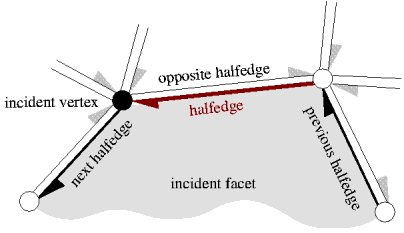
\includegraphics{halfedge_small.png}
					\caption{Structure d'un Polyhedron\_3}
				\end{figure}
				Il est ainsi possible d'accéder à partir d'un composant à tous les autres composants adjacents. Par exemple, halfedge()-\textgreater facet() permet d'accéder dans cette figure à la face qui contient la demi-arête en rouge.
				
			\subsection{Chargement d'un obj}
				Le premier obstacle a été de gérer le chargement d'un fichier de format obj et de le transcrire comme un Polyhedron\_3. En effet, CGAL ne gère pas nativement cette option, ayant préféré le format .off. Cependant, un développeur nommé James Greggson a publié sur son blog (http://jamesgregson.blogspot.fr) en mai 2012 une version de loader obj et transcrit en Polyhedron\_3. J'ai donc repris son code et l'ait amélioré pour gérer en plus la subdivision en plusieurs Polyhedrons s'il s'avère qu'un fichier .obj contenait plusieurs objets en eux-même (la version initiale du développeur chargeait tous les objets d'un fichier obj en un seul Polyhedron\_3). \par 
				De manière simple, CGAL peut incrémentalement créer un Polyhedron\_3, en déclarant un nouveau polyèdre par la fonction begin\_surface(nombre de sommets, nombre de faces). Ensuite, on ajoute chaque sommet avec la fonction add\_vertex(objet de type Point(x, y, z)). Enfin, on créé les faces du Polyhedron\_3. Pour chaque face à créer, on déclare la nouvelle face (avec begin\_facet()), on ajoute un à un les numéros de sommets dans l'ordre du fichier obj (avec add\_vertex\_to\_facet(num de la face)), puis on signale que la face à créer est terminée (avec end\_facet()), ce qui va relier le dernier sommet au premier. Il faut juste faire attention au fait que le format obj commence à l'indice 1, mais c++, comme de nombreux langages de développement, commence à l'indice 0.
			
			\subsection{Exporter un obj}
				De la même manière, il m'a fallu récupérer le fichier obj une fois le traitement du Polyhedron\_3 terminé. Étrangement, là où CGAL n'a pas prévu de manière native un chargeur obj, il a prévu un enregistreur, avec la fonction print\_polyhedron\_wavefront(). Il suffit juste d'exporter les polyèdres un par un dans un même fichier (via un ofstream), et on récupère ainsi un fichier obj prêt à l'emploi (par exemple pour le consulter via un logiciel adapté comme Blender).
		\section{Mailler un Polyhedron\_3}
			\subsection{Maillage initial}
				Le maillage d'un Polyhedron\_3 est constitué de ses faces. Ainsi, si un objet de type cube est importé avec un maillage triangulaire, il sera constitué de 12 faces, avec 2 faces dans le même plan pour chaque véritable face du cube.
			\subsection{Chercher la ou les faces du point d'impact}
				Comme indiqué dans l'algorithme 1, selon où se trouve le point d'impact, il faut agir différemment. En effet, si le point est sur une arête, alors il faut modifier le maillage des faces adjacentes afin de réaliser un impact sans modifier drastiquement la structure de l'objet. CGAL fournit toutefois un itérateur de faces, nommé Facet\_iterator, qui parcourt toutes les faces de l'objet 3D. Les faces de la scène 3D du pont Notre Dame étant toutes des triangles, il est possible de reconstruire un triangle avec pour coordonnées les points de la face. A partir de là, on vérifie si le point d'impact est sur le triangle. Si oui, on l'ajoute à un vecteur de faces. Sinon, on l'ignore. On reprend le processus jusqu'à la dernière face. Si le point d'impact est sur une arête, alors les deux faces qui composent l'arête seront détectées et ajoutées dans le vecteur de faces. La même chose sera appliquée pour un sommet, avec 3 faces ou plus d'ajoutées.
			\subsection{Cas d'un point sur une face}
				\subsubsection{Subdiviser la face}
					De nombreuses recherches et tentatives ont été effectuées pour subdiviser une face. \par
					Tout d'abord, j'ai commencé ma subdivision en effectuant une division barycentrique d'une face. Cette subdivision se fait en deux étapes. CGAL propose une fonction permettant de subdiviser une face du polyèdre, nommée create\_center\_vertex(pointeur d'halfedge de la face à subdiviser). Cette fonction relie tous les points de la face (Fig 2.1, halfedge de la face en rouge) vers un nouveau point créé de la face, qui sera placé au même endroit que le point pointé par l'halfedge initial, et retourne un Halfedge\_handle (un pointeur d'halfedge) partant de l'origine du halfedge passé en paramètre et pointant vers le nouveau point (Fig 2.2, l'halfedge retourné en bleu). A partir de là, on peut modifier la valeur du point du halfedge retourné en accédant au point (HalfedgeRetourné-\textgreater vertex()-\textgreater point()), et on le calcule en prenant la moyenne en x, y, et z, des trois points du triangle (Fig 2.3). Le problème majeur provient du fait que les triangles ainsi créés sont allongés par rapport au triangle original, et qu'à force de subdivision, les triangles seront de plus en plus allongés. Les impacts seront donc beaucoup trop étalés sur un côté, ce qui ne donnera pas un résultat sympathique. \par 
					\begin{figure}[h]
						\centering
						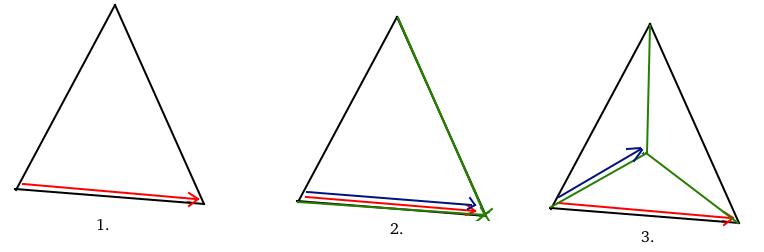
\includegraphics[width=1\textwidth]{FigBarycentricMesh.png}
						\caption{Subdiviser une face}
					\end{figure}
					\begin{figure}[h]
						\centering
						
\includegraphics[width=0.5\textwidth]{impact1.png}
						\caption{Impact sur une face d'un cube en 3 points}
					\end{figure}
					Ensuite je me suis tourné, avec l'avis de M. Rousselle, vers la triangulation de Delaunay, afin de pallier au problème des triangles allongés. Il est possible de réaliser cette triangulation via CGAL, mais pas avec un Polyhedron\_3, mais avec un MeshDomain\_3. Toutefois, par manque de temps, je n'ai pas pu approfondir les recherches à ce niveau. CGAL peut certainement proposer un moyen de convertir de l'un vers l'autre et réciproquement, auquel cas ce travail serait possible. De nouvelles recherches à ce niveau seront effectuées dans le cadre de mon stage afin d'améliorer la subdivision autour d'un point. \par
					J'ai toutefois trouvé un moyen de contourner le problème des triangles allongés. En effet, si chaque sous-triangle d'une face est elle-même divisée en 2, alors les triangles crées seront beaucoup moins allongés, car plus nombreux (6 au lieu de 3). CGAL prévoit aussi une fonction de division d'arêtes, nommée split\_edge(pointeur d'halfedge à subdiviser), qui fonctionne de la même manière que la fonction précédente. On créé avec la fonction le point qui sert de subdivision, puis on replace le point là où on le souhaite, dans mon cas, au milieu de l'arête. Le souci majeur de cette fonction est que le point n'est pas relié aux points des faces qui le relient. Mais ce problème est vite réglé, car en faisant l'appel à split\_edge() puis à create\_center\_vertex(), le point central créé va se relier aux sommets du triangle, mais aussi aux points créés sur les arêtes de ce triangle. Ainsi, au lieu de subdiviser une face en 3 triangles, on la subdivise en six, réduisant l'étirement des triangles (Figure 4). 
					\begin{figure}[h]
						\centering
						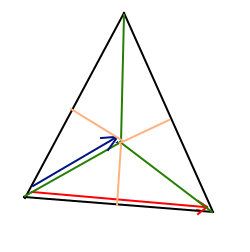
\includegraphics[width=0.3\textwidth]{FigBarycentricMeshSplit.png}
						\caption{Subdiviser une face en six points}
					\end{figure}
					\begin{figure}[h]
						\centering
						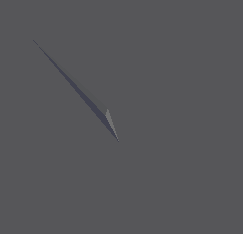
\includegraphics[width=0.5\textwidth]{impact2.png}
						\caption{Impact sur une face d'un cube en 6 points}
					\end{figure}
				\subsubsection{Supprimer les T-vertices}
					La dernière méthode de subdivision présentée pose un très gros problème : la formation d'arêtes en T. Concrètement, dans le cas de la figure 3, on peut voir que les 3 points au centre des arêtes créés forment un T. De nombreux algorithmes de traitement de lumière, entre autres, n'arrivent pas à gérer correctement ces cas, générant des artefacts désagréables. Le but est donc de prolonger la subdivision aux points d'arêtes afin d'éviter ces T vertices. \par 
					Une méthode simple appliquée dans mon cas a simplement été de rechercher les faces adjacentes, et de réaliser à leur tour une subdivision barycentrique sans subdiviser les arêtes qui ne le sont pas déjà. Ainsi, les arêtes subdivisées génèrent une arête de prolongation, et les autres ne généreront pas de T-vertices à leur tour. \par 
					Je rappelle que la structure du Polyhedron\_3 proposé par CGAL identifie les arêtes non pas comme des edges, mais comme des halfedges. Ainsi, l'halfedge opposé à celui de la face en cours (halfedge-\textgreater opposite()) concerne la même arête, mais cette fois, concerne la face de l'autre côté de l'arête, qui est donc adjacente à la face en cours de traitement. Rappeler la méthode de subdivision de faces, sur la face adjacente donc, permet de subdiviser la face adjacente, et donc de prolonger le point créé sur l'arête lors de la subdivision initiale.
				\subsubsection{Vérifier la taille de la face à impacter}
					Il faut maintenant vérifier si on doit raffiner le maillage ou non. Pour cela, on cherche la nouvelle face qui contient le point d'impact, on calcule la distance entre un point de la face trouvée et le point d'impact. Si la distance est supérieure à un certain seuil, on recommence les deux premières étapes. Sinon, on passe à la dernière étape. Cette vérification est en fait un appel récursif des deux premières étapes.
				\subsubsection{Impacter la face}
					Cette étape est en réalité la plus simple. En effet, nous avons déjà récupéré la face concernée par l'impact. Il suffit juste donc de créer un point au milieu de cette face, puis de déplacer le point créé de telle sorte qu'il créé une sorte de creux dans la face. \par
					En l'état, l'impact est créé "en dur", à savoir que je rentre moi même les coordonnées pour modifier l'objet. Toutefois, il est prévu par la suite, et conformément au papier de recherche Surface Aging by Impacts, de calculer la normale de la face qui sera impactée, et de déplacer le point créé dans le sens opposé à cette normale.
					Néanmoins, l'impact reste relativement étiré même avec la division en six sous-triangles. La triangulation de Delaunay reste une solution optimale à ce problème, et devra donc être traité le plus rapidement possible.
			\subsection{Cas d'un point sur une arête ou sur un sommet}
				N'ayant pas pu réaliser cette tâche, ceci ne concernera que la partie théorique. \par 
				L'idée est qu'en cas d'impact sur une arête, on puisse casser l'arête et créer un creux dans cette arête. Il faut donc :
				\begin{enumerate}
					\item Casser l'arête ciblée avec la fonction split\_edge()
					\item Casser les deux arêtes ainsi créées à proximité du point d'impact
					\item Utiliser la fonction create\_center\_vertex() sur les deux faces adjacentes et placer le point central à proximité du point d'impact (trouver un point à proximité est la raison pour laquelle cette section n'a pas été développée, car je n'ai pas encore trouvé de méthode optimale pour réaliser cette tâche)
					\item déplacer le point d'impact afin de créer un petit creux qui ne déforme pas tout l'objet, d'où la présence des 4 autres points.
				\end{enumerate}
				De la même manière, pour un sommet, il suffit de réaliser les même tâches, sans la première, car on déplacera directement le point "sommet" au lieu d'en créer un autre.
	\chapter{Perspectives}
		Par la suite, il est prévu de travailler sur les tâches suivantes : 
		\begin{itemize}
			\item Réaliser un impact sur une arête, puis sur un sommet, avec la méthode explicitée dans la section précédente.
			\item Permettre de réaliser un impact à partir d'un vecteur de frappe. Le point d'impact devra donc être calculé par l'intersection du vecteur généré et du polyèdre. 
			\item Améliorer le sous-maillage, non plus via une triangulation barycentrique, mais via la triangulation de Delaunay, afin de réduire l'étirement des triangles générés.
		\end{itemize}
		
	\chapter{Conclusion}
		Dans le cadre de ma période de projet, il m'a été demandé de réaliser un module de vieillissement d'un objet 3D, en simulant des impacts. Après diverses recherches, j'ai travaillé sur ce module en utilisant la bibliothèque CGAL, qui proposait l'objet Polyhedron\_3. \par
		J'ai ainsi pu réaliser une première version d'impact sur une face d'un objet, en affinant le maillage de l'objet 3D puis en ajoutant un point à proximité du point d'impact. Cependant, l'impact généré s'avère être trop étiré par rapport à la réalité, et l'affinage du maillage nécessite donc d'être retravaillé. \par
		Il reste encore du travail à faire après celà. En effet, les impacts peuvent avoir lieu sur les arêtes et sur les sommets d'un objet, auquel cas l'algorithme de travail devra être différent. \par
		Ces travaux complémentaires seront réalisés à l'occasion d'un stage en fin de Master 1.
	
	\newpage
\bibliographystyle{alpha}
\bibliography{biblio}
		
\end{document}

